\section{Einfache Bestimmung der Brennweite einer Linse}
\begin{table}[]
    \centering
    \begin{tabular}{|c|c|}
    	\hline
    	Messung Nr. & Pos. Linse (cm) \\
    	\hline
    	1 & 178.5 \\
    	\hline
    	2 & 178.4 \\
    	\hline
    	3 & 178.4 \\
    	\hline
    	4 & 178.4 \\
    	\hline
    	5 & 178.5 \\
    	\hline
    	6 & 178.4 \\
    	\hline
    	7 & 178.5 \\
    	\hline
    	8 & 178.3 \\
    	\hline
    	9 & 178.5 \\
    	\hline
    	10 & 178.5 \\
    	\hline
    
    \end{tabular}
    \caption{Daten: Einfache Bestimmung der Brennweite einer Linse}
    \label{tab:Daten1}
\end{table}


In diesem Versuchsteil soll die Brennweite einer Linse nur mit Hilfe eines Maßstabs und eines Schirms kontrolliert werden. Dazu wird sowohl die Linse als auch ein Schirm auf einer optischen Bank montiert \ref{fig:Versuch1.1}. Um den Fehler bei dieser Messung zu minimieren wird der Abstand zwischen Lichtquelle groß gewählt bzw. gegebenenfalls ein Kondensor nach der Lichtquelle zwischengeschaltet. Für die Messung wird nun die Linse solange verschoben, bis ein möglichst kleiner Lichtpunkt auf dem Schirm entsteht, der Abstand zwischen Schirm und der Linse ist somit die Brennweite. Für den Versuch wird eine Linse mit einer angegebenen Brennweite von $F = 15 cm$ gewählt, dabei wird der Schirm auf der 195cm-Marke der optischen Bank fixiert. Es ergeben sich die Werte in der Tabelle \ref{tab:Daten1}. Somit ergibt sich ein Mittelwert von $16.5600$ mit einer Standardabweichung von $0.066cm$, also: $16.5600cm \pm 0.066cm$. Was einer Abweichung von ca. $9 \% $ zum angegebenen Wert entspricht. Diese Abweichung kommt wahrscheinlich durch die ungenaue Messmethode zustande. Faktoren, die die Genauigkeit der Messung beeinflussen sind etwa, dass die Messung nicht mit monochromatischem Licht durchgeführt wurde und es somit zu einem anderen Ergebnis kommen könnte, da die Brechzahl auch von der Wellenlänge des Lichts abhängt. Allerdings wurden zehn dicht aneinander liegende Werte ermittelt, was eventuell auch auf eine nicht korrekte Angabe der Brennweite auf der Linse hindeuten könnte.

\begin{figure}
    \centering
    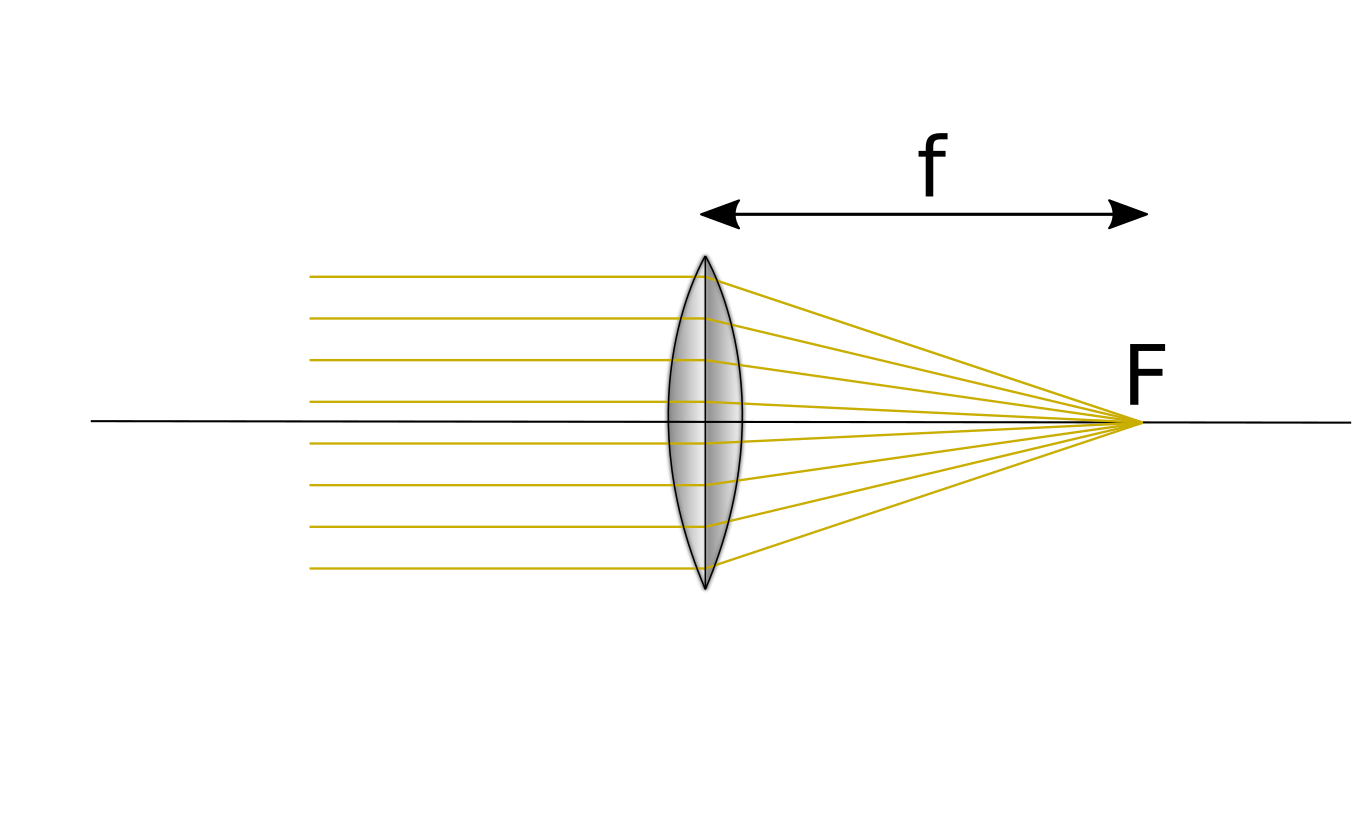
\includegraphics{Geometrische_Optik/Protokoll/fig/Versuch1.1.png}
    \caption{Einfach Bestimmung der Brennweite einer Linse}
    \label{fig:Versuch1.1}
\end{figure}

\section{Brennweitenbestimmung einer Linse mit dem Besselverfahren}

Zur genaueren Bestimmung der Brennweite einer dünnen Linse ist das Besselsche Verfahren gut geeignet. Dazu werden Bild (in unserem Fall ein Dia), Schirm und Linse wie auf der Skizze gezeigt angeordnet. Hierbei macht man sich zu Nutze, dass es bei einem festen Abstand zwischen Bild und Schirm zwei mögliche Linsenstellungen gibt, bei denen ein scharfes Bild auf den Schirm geworfen wird. Dies soll im folgenden durch die Herleitung gezeigt werden. Durch einsetzen der Relationen in Gleichung \ref{Relation} in die Linsengleichung \ref{Linsengleichung}, die leicht geometrisch einzusehen ist, erhält man, die Gleichung \ref{Gleichung}, diese Gleichung wird für $g$ gelöst, wobei die Differenz von $g_1$ und $g_2$ als e definiert wird \ref{Defe}, nach einer weiteren trivialen Umformung erhält man eine Gleichung für $f$ \ref{Gleichungf}.\\
Aus Gleichung \ref{Defe} ist direkt offentsichtlich, dass für eine reelles Ergebnis $a^2 \geq 4af$ gelten muss. Außerdem ist aus der gleichen Gleichung auch ersichtlich, dass es nicht vorteilhaft ist $\frac{e}{f}$ zu groß zu wählen, da im Grenzfall $e = a$ gilt und somit die Linse im Bild/Schirm stehen müsste. \\
Abgesehen von der eigentlichen Brennweitenbestimmung werden in diesem Versuchsteil auch zwei Linsenfehler genauer betrachtet: die chromatische und die sphärische Abberation. Dazu werden bei der Brennweitenmessung für die chromatische Rot- und Blaufilter und für die sphärische Abberation Ring- und Lochblende verwendet.\\
Bei der chromatischen Abberation handelt es sich um die Eigenschaft von Linsen aufgrund von Dispersion, also der Abhängigkeit der Brechzahl von der Wellenlänge, beispielsweise blaues Licht stärker zu brechen als rotes. Um diese zu messen werden Farbfilter verwendet und somit die Brennweite von blauem und rotem Licht unabhängig zu messen und somit die chromatische Abberation zu bestimmen.\\
Die sphärische Abberation ist ein Linsenfehler bei dem, im Normalfall, achsennahes Licht weniger stark gebrochen wird, als achsenfernes Licht, somit fällt die Brennweite für achsenahes Licht größer aus, als für achsenfernes Licht. Um diesen Linsenfehler qualitativ zu beschreiben werden Loch- und Ringblende vor der Linse fixiert und somit für achsennahes und achsenfernes Licht separat die Brennweiten gemessen.\\

\begin{equation} \label{Linsengleichung}
    \frac{1}{f} = \frac{1}{b} + \frac{1}{g}
\end{equation}

\begin{align} \label{Relation}
    b &= a - g   \\
    \nonumber b &= \frac{a-e}{2} 
\end{align}

\begin{equation} \label{Gleichung}
    \frac{1}{f} = \frac{a}{ag-g^2}
\end{equation}

\begin{equation} \label{Defe}
    e = \Delta g = \sqrt{a^2-4af}
\end{equation}

\begin{equation} \label{Gleichungf}
    f = \frac{a^2-e^2}{4a}
\end{equation}


\subsection{Fehlerrechnung zur Brennweitenbestimmung einer Linse mit dem Besselverfahren}


\section{Brennweitenbestimmung eines Zweilinsensystems mit dem Abbéschen Verfahren}

\subsection{Fehlerrechnung zur Brennweitenbestimmung eines Zweilinsensystems mit dem Abbéschen Verfahren}